\documentclass[12pt,a4paper]{article}

% 导入必要的宏包
\usepackage[UTF8]{ctex}
\usepackage{geometry}
\usepackage{amsmath}
\usepackage{amsfonts}
\usepackage{amssymb}
\usepackage{graphicx}
\usepackage{enumitem}
\usepackage{xcolor}
\usepackage{tikz}
\usepackage{float}
\usepackage{hyperref}
\usepackage{multicol}
\usepackage{longtable}
\usepackage{array}
\usepackage{tabularx}
\usepackage{listings}

% 代码高亮设置
\lstset{
    basicstyle=\ttfamily\small,
    keywordstyle=\color{blue},
    commentstyle=\color{green!70!black},
    stringstyle=\color{red},
    breaklines=true,
    numbers=left,
    numberstyle=\tiny\color{gray},
}

% 页面设置
\geometry{left=2.5cm,right=2.5cm,top=2.5cm,bottom=2.5cm}

% 标题页设置
\title{\textbf{2014年数据结构题库} \\ \large 单项选择题与综合应用题详解}
\author{}
\date{}

% 定义题型环境
\newenvironment{choicequestion}[1][]{%
    \vspace{0.5cm}
    \noindent\textbf{[#1]}
    \vspace{0.2cm}
}{}

\newenvironment{answersection}{%
    \vspace{0.2cm}
    \noindent\textbf{[参考答案]}\\
    \vspace{0.1cm}
}{}

\newenvironment{analysissection}{%
    \vspace{0.2cm}
    \noindent\textbf{[答案解析]}\\
    \vspace{0.1cm}
}{}

% 定义题号计数器
\newcounter{questioncounter}

% 定义题号计数器
\newcounter{questioncounter}

% 问题格式化命令
\newcommand{\question}[2]{%
    \stepcounter{questioncounter}%
    \noindent\textbf{\thequestioncounter} #1%
}

% 选择题选项格式
\newcommand{\choices}[4]{%
    \begin{multicols}
    \noindent \textbf{A.} #1 \par
    \noindent \textbf{B.} #2 \par
    \noindent \textbf{C.} #3 \par
    \noindent \textbf{D.} #4 \par
    \end{multicols}%
}

% 开始文档
\begin{document}

\maketitle

\section{单项选择题}

\begin{choicequestion}[单选题]
\question{下列程序段的时间复杂度是
$$
\begin{array}{l} 
\text{count} = 0; \\ 
\text{for (k = 1 ; k <= n ; k *= 2)} \\ 
\text{for (j = 1 ; j <= n ; j ++)} \\ 
\text{count ++ ;} 
\end{array}
$$}{}

\choices{$O(\log_2 n)$}{$O(n)$}{$O(n\log_2 n)$}{$O(n^2)$}

\begin{answersection}
C. $O(n\log_2 n)$
\end{answersection}

\begin{analysissection}
外层循环中 $k$ 从1开始，每次乘以2，直至 $k > n$，共执行 $\lfloor \log_2 n \rfloor$ 次。内层循环每次执行 $n$ 次。因此总时间复杂度为 $O(n \log_2 n)$。
\end{analysissection}
\end{choicequestion}

\begin{choicequestion}[单选题]
\question{假设栈初始为空，将中缀表达式 $\mathbf { a } / \mathbf { b } + ( \mathbf { c } * \mathbf { d } - \mathbf { e } * \mathbf { f } ) / \mathbf { g }$ 转换为等价的后缀表达式的过程中，当扫描到f时，栈中的元素依次是}{}

\choices{$+ ( * -$}{$+(−*$}{$/+(*-$}{$/+*-$}

\begin{answersection}
B. $+(−*$
\end{answersection}

\begin{analysissection}
中缀表达式 $a/b+(c*d-e*f)/g$ 转换为后缀表达式时，扫描到f时，栈中从底到顶的元素依次为+、-、*。此时已处理完括号内的*c*d-e*f*部分，+和-仍在栈中等待后续运算符。
\end{analysissection}
\end{choicequestion}

\begin{choicequestion}[单选题]
\question{循环队列放在一维数组 $\mathbf { A } [ 0 \ldots M - 1 ]$ 中，end1指向队头元素，end2指向队尾元素的后一个位置。假设队列两端均可进行入队和出队操作，队列中最多能容纳 $M-1$ 个元素。初始时为空。下列判断队空和队满的条件中，正确的是}{}

\choices{队空：end1 $== $ end2;\newline 队满：end1== (end2 + 1) mod M}{队空：end1 $= $ end2;\newline 队满：end2 == (end1 + 1) mod (M-1)}{队空：end2 $= $ (end1 + 1) mod M;\newline 队满：end1 $= = ( \mathbf { e n d } 2 + 1 )$ mod $M$}{队空：end1 $= = $ (end2 + 1) mod M;\newline 队满：end2 $=$ (end1 $+ 1$ ) mod (M-1)}

\begin{answersection}
A. 队空：end1 $== $ end2;\newline 队满：end1== (end2 + 1) mod M
\end{answersection}

\begin{analysissection}
循环队列通常预留一个空位置区分队空与队满。队空时队头指针等于队尾指针（end1==end2）；队满时队头指针等于队尾指针的下一个位置，即end1==(end2+1) mod M。
\end{analysissection}
\end{choicequestion}

\begin{choicequestion}[单选题]
\question{若对如下的二叉树进行中序线索化，则结点 $\mathbf { x }$ 的左、右线索指向的结点分别是}{}

\begin{figure}[H]
\centering
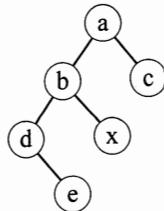
\includegraphics[width=0.3\textwidth]{images/9007ee03b96b96f437b0b600fb3750b046c1dae3d9ac3c700e1a2ab7a216b4d1.jpg}
\end{figure}

\choices{e、c}{e、a}{b、c}{b、a}

\begin{answersection}
D. b、a
\end{answersection}

\begin{analysissection}
中序遍历顺序为左-根-右。对图中二叉树进行中序遍历，结点x的前驱为b，后继为a。因此在中序线索化后，x的左线索指向b，右线索指向a。
\end{analysissection}
\end{choicequestion}

\begin{choicequestion}[单选题]
\question{将森林F转换为对应的二叉树T，F中叶结点的个数等于}{}

\choices{T中叶结点的个数}{T中度为1的结点个数}{T中左孩子指针为空的结点个数}{T中右孩子指针为空的结点个数}

\begin{answersection}
C. T中左孩子指针为空的结点个数
\end{answersection}

\begin{analysissection}
森林转换为二叉树采用“左孩子-右兄弟”表示法。森林中的叶结点在转换后的二叉树中没有左孩子（因无子女），但可能有右兄弟。因此F中叶结点的个数等于T中左孩子指针为空的结点个数。
\end{analysissection}
\end{choicequestion}

\begin{choicequestion}[单选题]
\question{5个字符有如下4种编码方案，不是前缀编码的是}{}

\choices{01,0000,0001,001,1}{011,000,001,010,1}{000,001,010,011,100}{0,100,110,1110,1100}

\begin{answersection}
D. 0,100,110,1110,1100
\end{answersection}

\begin{analysissection}
前缀编码要求没有任何一个编码是另一个编码的前缀。选项D中“110”是“1100”的前缀，违反前缀码定义。其余选项均满足前缀码条件。
\end{analysissection}
\end{choicequestion}

\begin{choicequestion}[单选题]
\question{对如下所示的有向图进行拓扑排序，得到的拓扑序列可能是}{}

\begin{figure}[H]
\centering
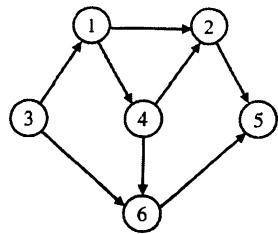
\includegraphics[width=0.3\textwidth]{images/ab8ef82dfe9b0507bffcfb02234958926d1f044e04c0e7cff737569e7e363530.jpg}
\end{figure}

\choices{3,1,2,4,5,6}{3,1,2,4,6,5}{3,1,4,2,5,6}{3,1,4,2,6,5}

\begin{answersection}
B. 3,1,2,4,6,5
\end{answersection}

\begin{analysissection}
拓扑排序需满足有向边的前驱后继关系。选项B中3在1之前，1在2之前，2在4之前，4在6之前，6在5之前，符合图中所有边的拓扑约束。其余选项存在违反先后顺序的情况。
\end{analysissection}
\end{choicequestion}

\begin{choicequestion}[单选题]
\question{用哈希（散列）方法处理冲突（碰撞）时可能出现堆积（聚集）现象。 下列选项中，会受堆积现象直接影响的是}{}

\choices{存储效率}{散列函数}{装填（装载）因子}{平均查找长度}

\begin{answersection}
D. 平均查找长度
\end{answersection}

\begin{analysissection}
堆积现象会导致同义词在散列表中连续聚集，使得查找时需进行更多探测，从而直接增加平均查找长度。
\end{analysissection}
\end{choicequestion}

\begin{choicequestion}[单选题]
\question{在一棵具有15个关键字的4阶B树中， 含关键字的结点个数最多是}{}

\choices{5}{6}{10}{15}

\begin{answersection}
D. 15
\end{answersection}

\begin{analysissection}
4阶B树中每个结点最多含3个关键字，最少含1个关键字（根结点除外）。要使结点数最多，需让每个结点含最少关键字（1个），故最多可有15个结点。
\end{analysissection}
\end{choicequestion}

\begin{choicequestion}[单选题]
\question{用希尔排序方法对一个数据序列进行排序时，若第1趟排序结果为9,1,4,13,7,8,20,23,15, 则该趟排序采用的增量（间隔）可能是}{}

\choices{2}{3}{4}{5}

\begin{answersection}
C. 4
\end{answersection}

\begin{analysissection}
希尔排序按增量划分子序列进行插入排序。若增量为4，则分为4组：(9,7,15)、(1,8)、(4,20)、(13,23)。对每组排序后结果为9,1,4,13,7,8,20,23,15，与题干一致。
\end{analysissection}
\end{choicequestion}

\begin{choicequestion}[单选题]
\question{下列选项中，不可能是快速排序第2趟排序结果的是}{}

\choices{2,3,5,4,6,7,9}{2,7,5,6,4,3,9}{3,2,5,4, 7,6,9}{4,2, 3,5,7,6,9}

\begin{answersection}
C. 3,2,5,4, 7,6,9
\end{answersection}

\begin{analysissection}
快速排序每趟确定一个基准元素的最终位置。第2趟结束后，最多有两个元素已确定最终位置。选项C中3和2相邻且顺序错误，5和4相邻且顺序错误，不符合快速排序的划分特性。
\end{analysissection}
\end{choicequestion}

\section{综合应用题}

\begin{choicequestion}[问答题]
\question{（13分）二叉树的带权路径长度(WPL)是二叉树中所有叶结点的带权路径长度之和。给定一棵二叉树T , 采用二叉链表存储， 结点结构为 left、weight、right，其中叶结点的weight域保存该结点的非负权值。设root为指向T的根结点的指针， 请设计求T的WPL的算法。要求：\newline
1)给出算法的基本设计思想。  \newline
2)使用C或C++语言， 给出二叉树结点的数据类型定义。  \newline
3)根据设计思想， 采用C或C++语言描述算法， 关键之处给出注释。}{}

\begin{answersection}
1）算法的基本设计思想：递归遍历二叉树，对每个叶结点将其权值乘以当前深度（路径长度）累加到WPL中。
\end{answersection}

\begin{analysissection}
2）二叉树结点数据类型定义：
\begin{lstlisting}[language=C]
typedef struct BiTNode {
    struct BiTNode *left;
    int weight;          // 叶结点保存权值，非叶结点可为0
    struct BiTNode *right;
} BiTNode, *BiTree;
\end{lstlisting}

3）算法实现：
\begin{lstlisting}[language=C]
int WPL(BiTree root, int depth) {
    if (root == NULL) return 0;
    if (root->left == NULL && root->right == NULL) {
        return root->weight * depth;   // 叶结点贡献
    }
    return WPL(root->left, depth + 1) + WPL(root->right, depth + 1);
}

int calculateWPL(BiTree root) {
    return WPL(root, 0);   // 从根开始，深度为0
}
\end{lstlisting}
\end{analysissection}
\end{choicequestion}

\end{document}